\documentclass[12pt,fleqn]{article}
\setlength{\parindent}{0pt}
\usepackage{graphicx}
\usepackage{listings}
\usepackage[latin5]{inputenc}
\setlength{\parskip}{8pt}
\setlength{\parsep}{0pt}
\setlength{\headsep}{0pt}
\setlength{\topskip}{0pt}
\setlength{\topmargin}{0pt}
\setlength{\topsep}{0pt}
\setlength{\partopsep}{0pt}
\setlength{\mathindent}{0cm}

\begin{document}
MIT OCW Cok Degiskenli Calculus - Ders 2

Onceki derste iki uygulama gorduk. Ucuncu bir uygulama bir $\vec{A}$
vektorunun bir birim vektor $\vec{u}$ yonundeki bilesenlerini /
parcalarinin (components) hesaplanmasidir.

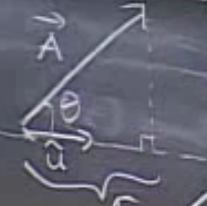
\includegraphics[height=3cm]{2_1.png}

Ustteki sekilde $\vec{A}$'nin $\vec{u}$ yonundeki ``yansimasini'' goruyoruz
ve bu yansima $\vec{A}$'nin $\vec{u}$ yonundeki bilesenidir,
buyuklugudur. 

Aradaki a�� $\theta$ ise ve ucgen dik ise, o zaman bu yansima 

\[ |\vec{A}| cos(\theta) \]

olarak hesaplanacaktir. Bu formulun ilk hali aslinda

\[ |\vec{A}| |\vec{u}| cos (\theta) \]

fakat $\vec{u}$ birim vektor olduguna gore, uzunlugu 1, o zaman bu buyukluk
carpimdan atilabilir.  Ustteki formul ayni zamanda bir noktasal carpim,
$\vec{A}\cdot\vec{u}$.

Eger bir vektorun mesela $\hat{i}$ yonundeki yansimasini almak isteseydik,

\[ \vec{A} \cdot \hat{i} \]

kullanirdik, bu da

\[ \vec{A} \cdot <1,0,0>\]

olurdu. Bu carpim $x$ yonunde 1 ile carpar diger tum eksenleri sifirlar,
yani diger bir degisle $\vec{A}$'nin $x$ yonundeki bilesenini hesaplamis oluruz. Bu
arada $\hat{i}$ tabii ki bir birim vektor. Uzunlugu 1.

Uygulama 

Fizikte, yuvarlak bir sekilde donebilen bir sarkac problemini dusunelim. Bu
sistemi analiz etmek icin Newton Kanunu, mekanik, vs. kullanmaniz gerekir
tabii ki, fakat vektorler  geometrik olarak bu sistemi anlamak icin cok
faydalidir. 

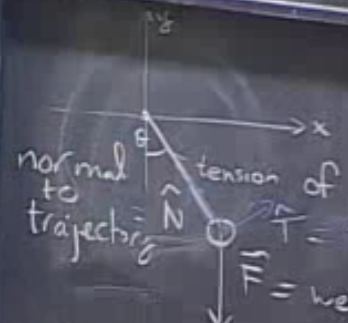
\includegraphics[height=4cm]{2_2.png}

Bu sarkacin ileri geri sallanmasinin sebebi ustte takip edilen yuvarlak
yoldur. Analiz icin $x, y$ yonundeki bilesenlere bakmak yerine belki de
resimdeki iki birim vektor yonune bakmamiz lazim, ki bu vektorlerden biri
takip edilen yola teget yonu gosteren $\vec{T}$, digeri yuvarlak tanjantina
dik olan $\vec{N}$. O zaman agirligi temsil eden $\vec{F}$'in bu iki vektor
yonundeki bilesenlerine bakabiliriz.

Resimde ipin gerginligi (tension of string) $\vec{N}$ yonunde, bu yon ip
gerginligi yonu, $\vec{F}$'in $\vec{N}$ yonundeki bileseni gerginligi
yaratan faktordur. $\vec{F}$'in tegetlik yani $\vec{T}$ yonundeki bileseni ise
ileri geri hareketi saglayan faktordur.

Muhakkak sarkacin $y$ ekseni ile olusturdugu bir a�� $\theta$ uzerinden bir
suru cos, sin terimleri iceren denklemler ortaya cikartabilirdiniz, bu
ilginc olurdu, fakat eger daha kisa bir yolu takip etmek istiyorsak,
noktasal carpim kullaniriz. 

Vektorler baglaminda anlamamiz gereken bir diger kavram, alan
kavrami. Diyelim ki elimizde bir pentagon sekli var. Bu seklin alanini
vektorler kullanarak hesaplayabilir miydik? 

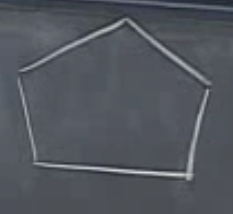
\includegraphics[height=2cm]{2_3.png}

Evet hesaplayabiliriz. Problemi basitlestirelim. Pentagonu ucgenlere
ayiralim. 

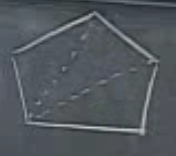
\includegraphics[height=2cm]{2_4.png}

sonra bu alanlari toplayalim. Ucgen alanini nasil hesaplariz? Soyle bir
ucgen dusunelim

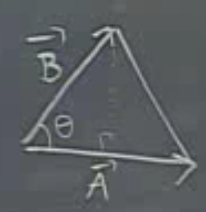
\includegraphics[height=2cm]{2_5.png}

Bu ucgenin alani

\[ \frac{1}{2}|\vec{A}||\vec{B}|sin(\theta) \]

Bu formul $cos$ iceren diger formulumuze benziyor. Bundan istifade
edebiliriz belki. Once $cos(\theta)$'yi buluruz, sonra $sin^2\theta + cos^2\theta
= 1$ esitligini 
kullanarak $sin(\theta)$'yi buluruz.

Fakat bu gereginden fazla is yaratir. Daha kolay bir yontem var. Bu yontem
icin determinantlar kullanmak lazim. 

Devam edelim: Madem a��larin cos degerlerini bulmayi biliyoruz, belki oyle
bir diger a�� bulmaliyiz ki o a��nin cos degeri bizim aradigimiz a��nin sin
degeri olsun, cunku alan icin sin gerekiyor, ama hesaplayabildigimiz cos. 

Birbirini tamamlayici a��lar (complemantary angles) kavramini biliyoruz
herhalde. 

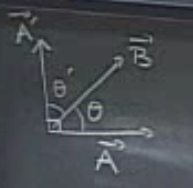
\includegraphics[height=3cm]{2_6.png}

Diyelim ki elimizde $\vec{A}$ var, onu $90^o$ cevirip ustteki hale getiriyoruz,
yeni vektore $\vec{A'}$ diyelim. O vektor ile $\vec{B}$ arasindaki a��ya da
$\theta'$ diyelim. 

\[ \theta' = \frac{\pi}{2} - \theta \]

\[ cos(\theta') = sin(\theta) \]

Bu demektir ki 

\[ |\vec{A}||\vec{B}|sin\theta = |\vec{A'}||\vec{B}|cos\theta'  \]

$|\vec{A}|$ yerine $|\vec{A'}|$ koymakla hicbir sey degistirmiyorum cunku
bu vektorlerin yonleri degisik olsa da buyuklukleri ayni. Devam edelim,
ustteki formulde sag tarafi basitlestirirsek

\[ = \vec{A'} \cdot \vec{B} \]

Bu temiz bir formul. Tek eksik, $\vec{A'}$'nin ne oldugunu hala
hesaplamadik. Fakat bunu yapmak o kadar zor degil. Bunun icin $\vec{A}$'yi
cevirebilmemiz lazim. Alttaki resme bakalim, 

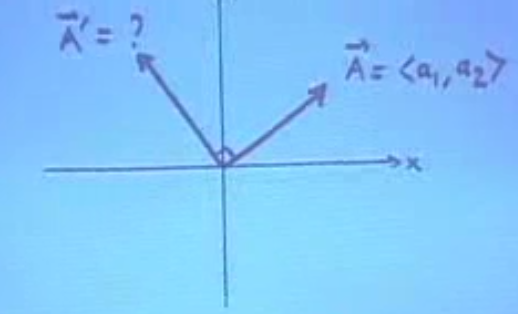
\includegraphics[height=4cm]{2_7.png}

acaba $\vec{A'}$ ne olur?  Secenekler [bu hoca boyle ufak sinavlari
seviyor, faydali aslinda, bu sinavlara gelince siz de cevabini vermeye
ugrasin].

\begin{enumerate}
   \item $<a_2,a_1>$
   \item $<a_2,-a_1>$
   \item $<-a_2,a_1>$
   \item $<-a_1,a_2>$
   \item Hicbiri
\end{enumerate}

Dogru cevap: 3. 

Bu nasil oldu? Alttaki resme bakalim

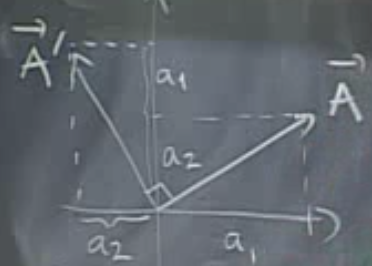
\includegraphics[height=4cm]{2_8.png}

$\vec{A}$'nin etrafinda bir dikdortgen hayal edelim, ve dikdortgeni
icindeki vektor ile beraber alip sola dogru ceviriyoruz. O zaman uzun kenar
artik yukari dogru bakiyor, yani $a_1$ yukari bakiyor, $a_2$ nin de yeri
degisiyor, yani bu buyuklukler yer degistiriyorlar. Ayrica $a_2$ artik ters
yone gittigi icin isareti degisiyor.

O zaman su formule donersek

\[ = \vec{A'} \cdot \vec{B} \]

soyle olur

\[ a_1b_2 - a_2b_1 \]

Bu formul determinantlardan tanidik gelebilecek bir formul, 

\[ = det(\vec{A},\vec{B}) \]

Aslinda $\vec{A},\vec{B}$ ile bu vektorleri yanyana kolonlara koydugumuz su
formu dusunuyoruz ve onun determinantini aliyoruz

\[ =
\left|\begin{array}{rr}
a_1 & a_2 \\
b_1 & b_2 \\
\end{array}\right|
 \]

Ve bu determinant hesabinin sonucu kenarlari $\vec{A}$ ve $\vec{B}$ olan
bir paralelogramin alanidir. Tabii paralelogram icindeki ucgeni istiyorsak
bu sonucu ikiye boleriz. 

Not: Alan pozitif bir seydir, fakat $a_1b_2 - a_2b_1$'in kesinlikle pozitif
cikmasinin garantisi yoktur. Eksi degerli terimler buyuyup arti degerlileri
asabilirler. O zaman ifadelerimizin tam dogru olmasi icin ustteki
determinant hesabi -alan ya da +alan degerine esittir demek lazim. 

Ilerleyelim

Uzayda (3 boyutta, kordinat sisteminde, vs.) yapabilecegimiz iki tur hesap
var. Bunlar objelerin ya dis alan hesabi (surfaces) ya da objelerin hacim
(volume) hesabi. Daha kolay olanla baslayalim, hacim hesabi.

Iddia ediyorum ki bu is icin uzay ortaminda kullanilabilecek bir tur
determinant var. Elimizde uc vektor $\vec{A},\vec{B},\vec{C}$ var ve bu vektorlerin
determinanti

\[ det(\vec{A},\vec{B},\vec{C}) = 
\left|\begin{array}{rrr}
a_1 & a_2 & a_3 \\
b_1 & b_2 & b_3 \\
c_1 & c_2 & c_3 
\end{array}\right|
 \]

\[ = 
a_1
\left|\begin{array}{rr}
b_2 & b_3 \\
c_2 & c_3
\end{array}\right|
-
a_2
\left|\begin{array}{rr}
b_1 & b_3 \\
c_1 & c_3
\end{array}\right|
+
a_3
\left|\begin{array}{rr}
b_1 & b_2 \\
c_1 & c_2
\end{array}\right|
\]

Ustteki gibi 2 x 2 determinantlarin acilimi biliyoruz zaten. O acilimi
ustteki formul icin yapinca elimize 6 tane terim gecmis olacak. Ustteki
formulu, yani bir 3 x 3 determinantin 2 x 2 acilimini hatirlamanin kisa
yolu nedir? Ustte kullandigimiz 1. satira gore acilim. 1. satirda sirayla
gideriz, $a_1$'e bakariz, onun oldugu satiri ve kolonu (zihnimizde) sileriz
ve geriye kalan 2 x 2 determinanti hemen hesaplariz. Boyle devam
ederiz. Ayrica ikinci 2 x 2 determinantin onunde bir eksi isareti olduguna
dikkat. Bunun niye oldugunun matematiksel sebebine burada girmeyecegiz.

Peki bu formul bize ne saglayacak? Su teoriyi saglayacak:

Teori

Geometriksel olarak $det(\vec{A},\vec{B},\vec{C}) = \pm \textrm{
  paralelipipe'in hacmi}$. 
Paralelipipe nedir? Bu obje bir nevi paralelogramin 3 boyuttaki hali. 
Alttaki gibi

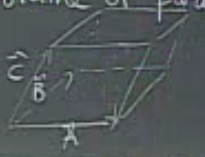
\includegraphics[height=2cm]{2_9.png}

Capraz Carpim (Cross Product)

Tanim

\[ \vec{A} \times \vec{B} =
\left|\begin{array}{rrr}
\hat{i}& \hat{j}& \hat{k} \\
a_1 & a_2 & a_3 \\
b_1 & b_2 & b_3 
\end{array}\right|
 \]

seklindedir ve bu islemin sonucu bir vektordur. Bu noktasal carpimdan
farkli, o sonuc bir tek sayiydi. Burada sonuc bir vektor.

Fakat bu determinant biraz garip. Icindeki elementler $\hat{i}$, $\hat{j}$
gibi birim vektorler. Bu tur determinantin ogeleri tek sayilar degil midir?
Ama aslinda amac $\hat{i}$'yi oldugu gibi hesaba dahil etmek degil, bu bir
notasyon sadece, boylece acilimi yaptigimizda

\[ = 
\left|\begin{array}{rr}
b_2 & b_3 \\
c_2 & c_3
\end{array}\right| 
\hat{i}
-
\left|\begin{array}{rr}
b_1 & b_3 \\
c_1 & c_3
\end{array}\right|
\hat{j}
+
\left|\begin{array}{rr}
b_1 & b_2 \\
c_1 & c_2
\end{array}\right|
\hat{k}
\]

$\hat{i}$, $\hat{j}$, $\hat{k}$'nin nereye gidecegini hatirlamak kolay oluyor.

Teoriler

1)

$|\vec{A} \times \vec{B}|$ bu vektorlerin olusturdugu paralelograminalanina esittir. Yani 
alan hesabi icin capraz carpimi yapariz, bir vektor elde ederiz, sonra bu 
vektorun uzunlugunu buluruz (tum ogelerinin karesini alip toplariz, 
karekok aliriz, vs). Burada arti, eksi ile ugrasmamiza gerek
yok cunku bir vektorun buyuklugu hep pozitiftir.

Yani dersin ilk kismiyla baglamak gerekirse, aslinda $det(\vec{A},\vec{B})
= |\vec{A} \times \vec{B}|$ 
demis oluyoruz. Kontrol edelim. Capraz carpim soyle

\[ \vec{A} \times \vec{B} =
\left|\begin{array}{rrr}
\hat{i}& \hat{j}& \hat{k} \\
a_1 & a_2 & a_3 \\
b_1 & b_2 & b_3 
\end{array}\right|
 \]

Determinant formulunu hatirlayalim

\[ = det(\vec{A},\vec{B}) \]

\[ =
\left|\begin{array}{rr}
a_1 & a_2 \\
b_1 & b_2 \\
\end{array}\right|
 \]

Bu formulde sadece $a_1,a_2,b_1,b_2$ var, o zaman capraz carpimi o hale
getirmek icin $a_3=0,b_3=0$ kullanabiliriz, cunku iki vektoru her zaman
alip xy duzlemi uzerine koyabiliriz [1]. Acilimi yaptimiz zaman
determinant sonucu ile ayni seyi elde ettigimizi goruruz.

2)

Sadece buyukluk degil, $\vec{A} \times \vec{B}$ degerinin yonu de cok ilginc. $dir(\vec{A} \times \vec{B})$ 
paralelogramin uzerinde oldugu duzleme tam dik yonu gosteriyor. 
Yani $\vec{A} \times \vec{B}$ ikisinin ciktigi noktadan, bu iki vektore de
dik olan 3. bir vektoru yaratir


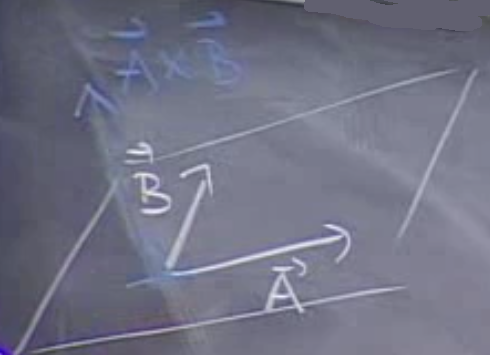
\includegraphics[height=3cm]{2_10.png}

Peki $\vec{A} \times \vec{B}$ hesabinin hangi yonde bir vektor yaratacagini
nereden bilecegiz? Sag el kuralini kullanarak.

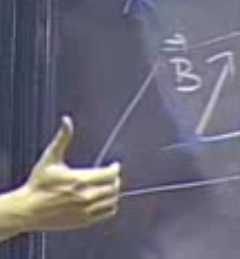
\includegraphics[height=3cm]{2_11.png}

Bu kurala gore el $\vec{A}$ yonunu gosterecek sekilde tutulur, parmaklar
bukulerek $\vec{B}$ yonune cevirilir. Bu haldeyken basparmak kaldirilir, ve
bu basparmak $\vec{A} \times \vec{B}$'nin yonunu gosterecektir.

Soru

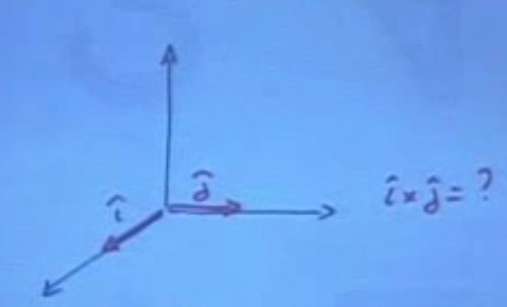
\includegraphics[height=4cm]{2_12.png}

Secenekler

\begin{enumerate}
   \item $\hat{k}$
   \item $-\hat{k}$
   \item $1$
   \item $0$
   \item Bilmiyorum
\end{enumerate}

Dogru cevap?

Cevap 1. Yani $\hat{i} \times \hat{j} = \hat{k}$

Kontrol edelim. 

\[ 
\left|\begin{array}{rrr}
\hat{i}& \hat{j}& \hat{k} \\
1 & 0 & 0 \\
0 & 1 & 0 \\
\end{array}\right| = 
0 \hat{i} - 0 \hat{j} - 1 \hat{k}  = 
\hat{k}
 \]

Hakikaten de sonuc sag el kuralini kullansak basparmagimizin gosterecegi
yon olan $\hat{k}$'yi gosteriyor. 

Simdi hacim hesabina geri donelim. Determinant kullanmadan nasil hacim
hesabi yaparim? 

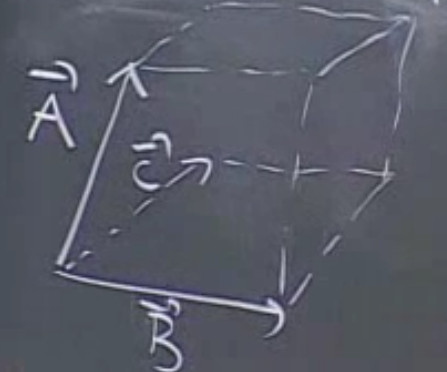
\includegraphics[height=4cm]{2_13.png}

Parallelipipe'nin hacminin taban alani carpi yuksekligi oldugunu biliyoruz
herhalde. Alan nedir? Tabanin kenari olan $\vec{B}$, ve $\vec{C}$'yi
kullaniriz, onlarin capraz carpimini aliriz, yani $\vec{B}\times
\vec{C}$. Fakat capraz 
carpimin sonucunun bir baska vektor oldugunu
soylemistik, o zaman o vektorun sadece buyuklugunu kullaniriz, $|\vec{B}\times
\vec{C}|$. 

Peki yuksekligi nasil hesaplariz? Yuksekligi en azindan yonsel olarak, bir
birim vektor olarak bildigimizi varsayalim, ve bu birim vektor $\vec{n}$
olsun. O zaman $\vec{A}\cdot\vec{n}$ yuksekligi hesaplayabilirdik. Soyle.

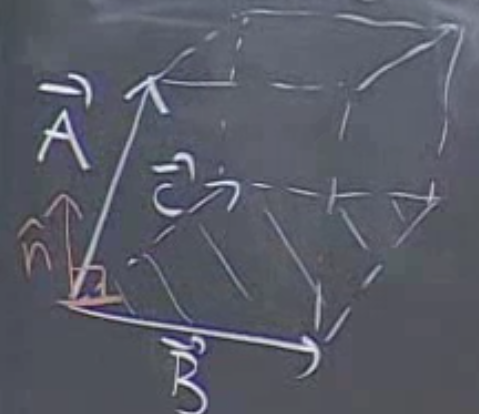
\includegraphics[height=4cm]{2_14.png}

Peki $\vec{n}$'i nasil hesaplariz?  $\vec{B}\times \vec{C}$ yukseklik
yonunde ucuncu bir vektor uretmez mi? Bu vektor $\vec{n}$ ile ayni yonde
olmaz mi? O zaman $\vec{B}\times \vec{C}$'yi kullanirim. Ama bu carpim
birimsel degildir, o zaman onu kendi buyuklugu ile bolerim, ve istedigim
birim vektoru elde ederim.

\[ \vec{n} = \frac{\vec{B}\times \vec{C}}{|\vec{B}\times \vec{C}|} \]

O zaman

\[ |\vec{B}\times \vec{C}| \vec{A}\cdot\vec{n} \]

\[  = |\vec{B}\times \vec{C}| \vec{A}\cdot \frac{\vec{B}\times \vec{C}}{|\vec{B}\times \vec{C}|}  \]

\[  = \vec{A}\cdot (\vec{B}\times \vec{C})  \]

Isin ilginci $det(\vec{A},\vec{B},\vec{C})$'nin ustteki formulle ayni sonucu vermesidir. 

Kaynaklar

[1] Anton, Rorres, Elementary Linear Algebra with Applications, 9th Edition


\end{document}
